
%%% Local Variables: 
%%% mode: latex
%%% TeX-master: t
%%% End: 

%%%%%%%%%%%%%%%%%%%%%%%%%%%%%%%%%%%%%%%%%%%%%%%%%%%%%%%%%%%%%%%%%%%%%%%%%
\section{Selection of the patient data}
%%%%%%%%%%%%%%%%%%%%%%%%%%%%%%%%%%%%%%%%%%%%%%%%%%%%%%%%%%%%%%%%%%%%%%%%%
\begin{figure}[ht]
\begin{center}
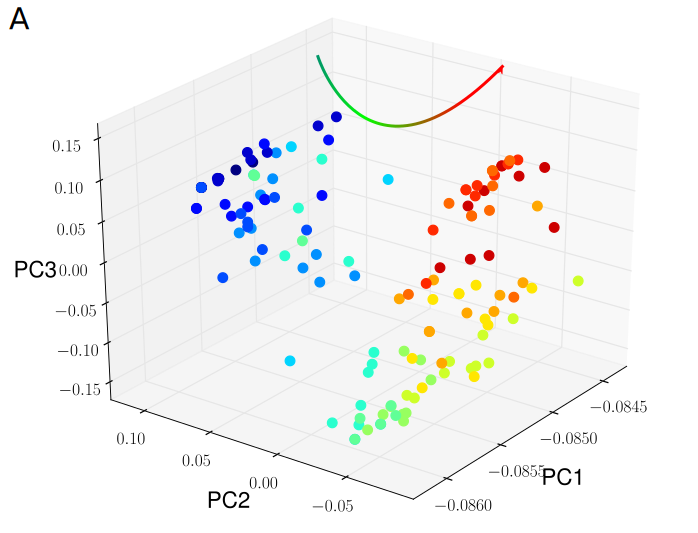
\includegraphics[width=0.35\linewidth]{Shankarappa_PCA_p1}
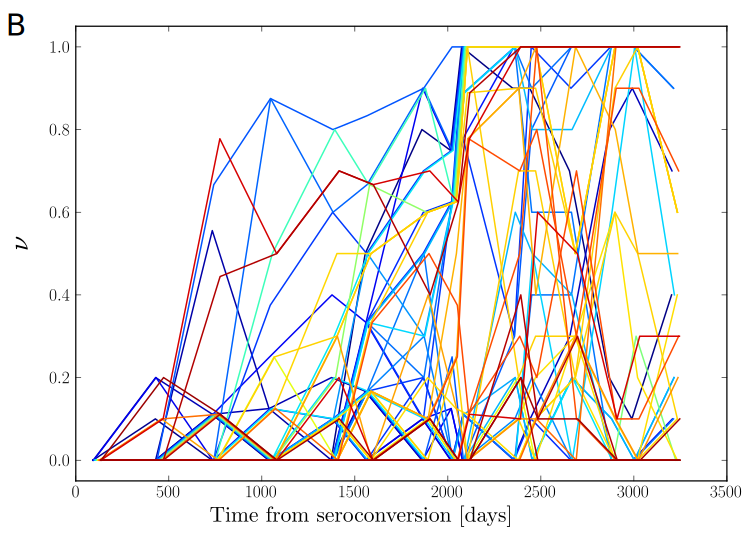
\includegraphics[width=0.35\linewidth]{Shankarappa_allele_freqs_trajectories_nonsyn_p1}
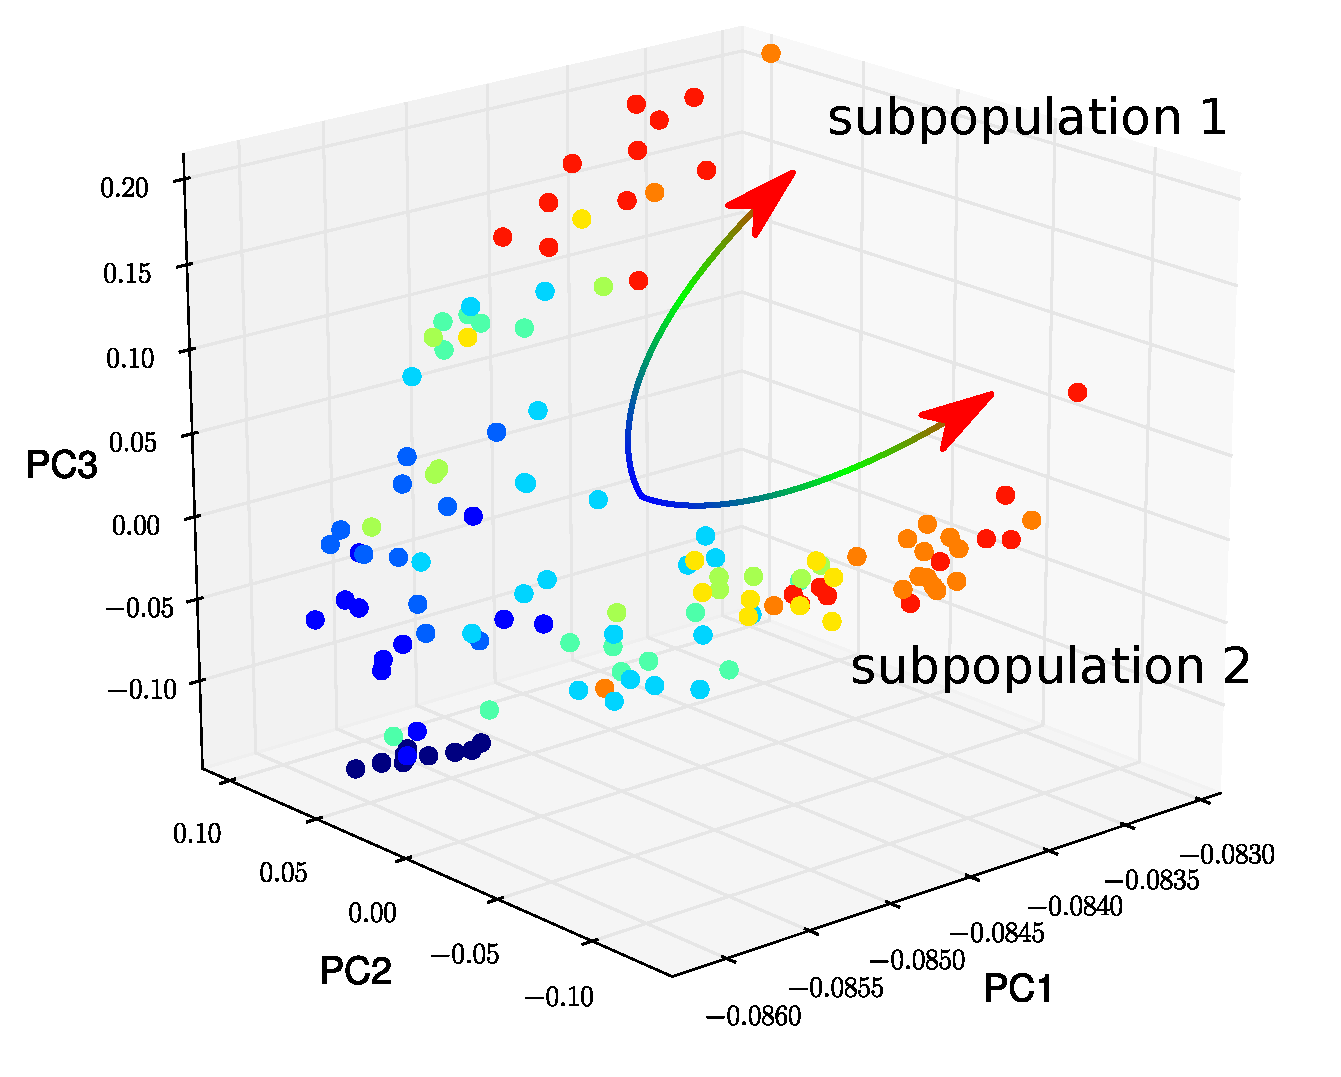
\includegraphics[width=0.35\linewidth]{Shankarappa_PCA_p7}
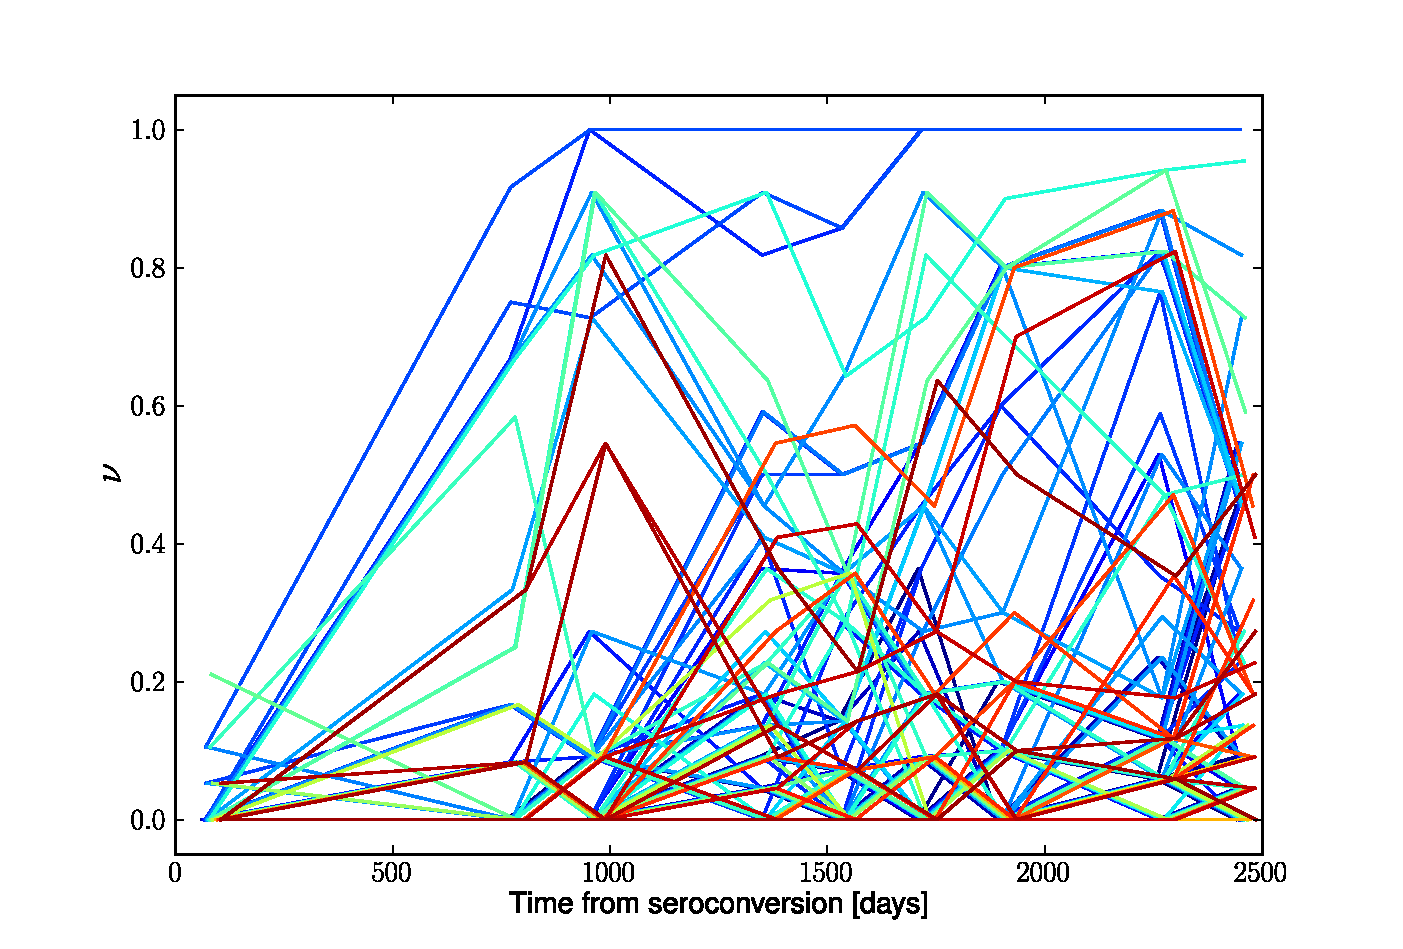
\includegraphics[width=0.35\linewidth]{Shankarappa_allele_freqs_trajectories_nonsyn_p7}
\caption{Structure of viral populations and patient selection.
Panel A) shows a PCA of all sequences from patient p1 (colors indicate time from
seroconversion, from blue to red). Panel B) Allele frequency trajectories for nonsynonymous
changes in the same patient. Here, the blue to red color map corresponds to the
position of the allele in \env{} from 5' to 3'. Panels C and D) show analogous
plots for data from patient p7. Samples after day 1000 split into two clusters in the PCA and no mutations that arise after day 1000 fix, presumably because they are restricted
to one subpopulation. All patients like p7 (p4, p7, p8, p9 from ref.~\citealp{shankarappa_consistent_1999} and
ACH19542 and ACH19768 from ref.~\citealp{bunnik_autologous_2008}) were excluded
from our analysis.}
\label{fig:aftp}
\end{center}
\end{figure}

\newpage
% %%%%%%%%%%%%%%%%%%%%%%%%%%%%%%%%%%%%%%%%%%%%%%%%%%%%%%%%%%%%%%%%%%%%%%%%
\section{Synonymous diversity across the HIV genome}
% %%%%%%%%%%%%%%%%%%%%%%%%%%%%%%%%%%%%%%%%%%%%%%%%%%%%%%%%%%%%%%%%%%%%%%%%
\begin{figure}[h]
\begin{center}
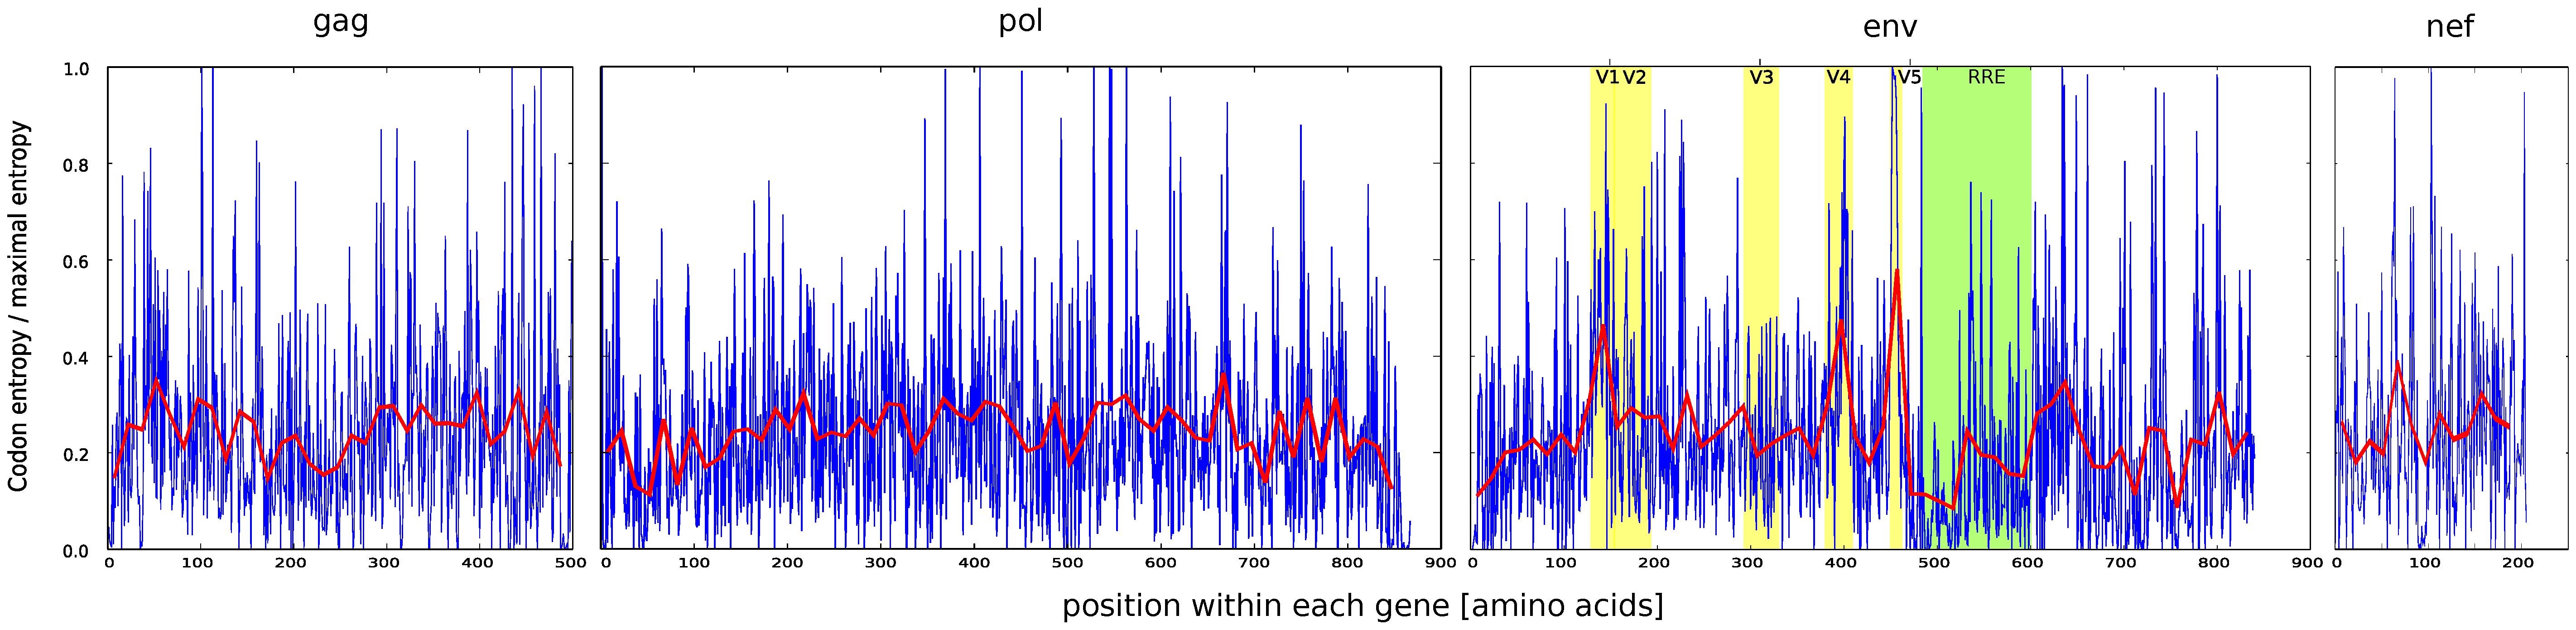
\includegraphics[width=\linewidth]{conservation_codons_genome}
\caption{
Synonymous diversity across the HIV genome, as quantified by the normalized
codon entropy among sequences coding for the consensus amino acid. In most
parts of the genome, synonymous sites show little conservation. The synonymous
diversity peaks at the variable regions in {\it env} and is reduced in regions 
under purifying selection (RRE hairpin, second {\it tat}/{\it rev} exons). The
normalized codon entropy is calculated as follows (see the script
\texttt{codon\_entropy\_synonymous\_subtypeB.py} for the full algorithm): (i)
from a subtype B multiple sequence alignment (MSA) from the LANL website (filtered sequences only, version 2011)~\cite{LANL2012}, we calculate the
consensus amino acid at each position in the HIV genome; (ii) we count how often
each codon coding for the consensus amino acid appears in the MSA; (iii) at each
amino acid position, we divide by the number of sequences in the MSA that had
the consensus amino acid at that position, obtaining {\it codon frequencies}
$\nu_c$; (iv) we calculate the codon entropy from each position as: $S := -
\sum_{c} \nu_c \log \nu_c$, where $c$ runs over codons that code for the
consensus amino acid at this site; (v) we divide by the maximal codon entropy of
that amino acid (e.g. $\log 2$ for twofold degenerate codons). All parts of
{\it env} that are part of a different gene (signaling peptide, second {\it rev}
exon) have been excluded from our main analysis, to avoid contamination by
protein selection in a different reading frame.
Note that all gap-rich columns of the MSA are stripped from this figure, hence genes such as {\it env} might appear shorter than they actually
are.
}
\label{fig:syndiv_genome}
\end{center}
\end{figure}
\newpage
% 
% %%%%%%%%%%%%%%%%%%%%%%%%%%%%%%%%%%%%%%%%%%%%%%%%%%%%%%%%%%%%%%%%%%%%%%%%%
% \section{Nonsynonymous changes outside of variable regions are deleterious}
% %%%%%%%%%%%%%%%%%%%%%%%%%%%%%%%%%%%%%%%%%%%%%%%%%%%%%%%%%%%%%%%%%%%%%%%%%
% \begin{figure}[h]
% \begin{center}
% 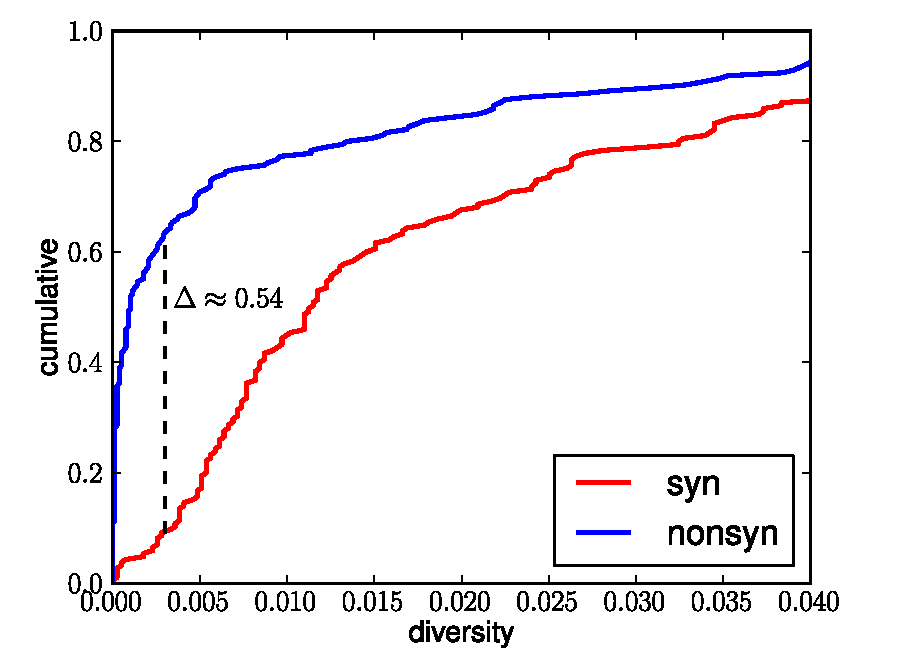
\includegraphics[width=0.8\linewidth]{synmut_conservation_4fold_synnonsyn}
% \caption{Cumulative distribution of synonymous and nonsynonymous diversity in
% {\it gag} in the LANL reference panel (filtered
% sequences only, version 2011)~\cite{LANL2012}. Sites such that the consensus codon
% has three synonymous and six nonsynonymous single mutants were used, and the number of observed mutants
% of a certain type over the number of possible mutants is plotted. Nonsynonymous
% changes are observed less often, {\it ergo} are more conserved, than
% synonymous changes. It can be therefore assumed, as mentioned in the main text,
% that non-escape nonsynonymous changes involve a large fitness cost.}
% \label{fig:synnonsyncons}
% \end{center}
% \end{figure}
% \newpage

%%%%%%%%%%%%%%%%%%%%%%%%%%%%%%%%%%%%%%%%%%%%%%%%%%%%%%%%%%%%%%%%%%%%%%%%%
\section{Time-dependent selection}
%%%%%%%%%%%%%%%%%%%%%%%%%%%%%%%%%%%%%%%%%%%%%%%%%%%%%%%%%%%%%%%%%%%%%%%%%
\begin{figure}[h]
\begin{center}
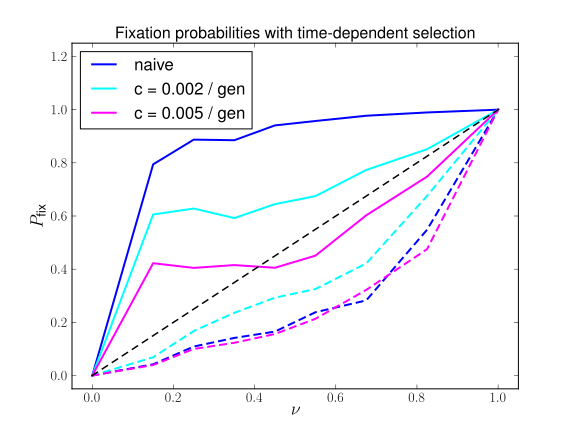
\includegraphics[width=0.6\linewidth]{simulations_gradually_timeselec_deadagain}
\caption{
Time-dependent selection reduces fixation of nonsynonymous mutations. The figure
compares the fixation probability in the time independent model (na\"ive) to
a model with time dependent selection that mimics the an evolving immune system.
It has been found that virus is typically neutralized by serum from a few month
earlier~\citep{richman_rapid_2003} but not by contemporary serum. We model this
evolving immune system by assuming that escaped variants loose their beneficial
effect with a rate proportional to the frequency of the escaped variant. 
Specifically, the selection effect of the escape mutations is
reset to its fitness cost of $-0.02$ with probability
\[ P_\text{recognized}(t) = c \cdot \nu(t), \] 
per generation, where $c$ is a constant coefficient shown in the legend that
encodes the overall efficiency of the host immune system. With increasing
probability of recognition, the fixation of frequent escape mutants is reduced,
while hitch-hiking of synonymous mutations is not affected. The precise
shape of $\pfix(\nu)$ depends on the details of the $P_\text{recognized}(t)$ and 
we do not think that the high $\pfix(\nu)$ for $\nu<0.2$ is meaningful.
The other parameters for the shown simulations are
the following: deleterious effect $s_d = 10^{-3}$, average escape rate $\epsilon = 0.016$,
fraction of deleterious synonymous mutations $\alpha = 0.986$, rate of new epitopes
$k_A=0.0014$ per generation.
}
\label{fig:tds}
\end{center}
\end{figure}

\newpage
%%%%%%%%%%%%%%%%%%%%%%%%%%%%%%%%%%%%%%%%%%%%%%%%%%%%%%%%%%%%%%%%%%%%%%%%%
\section{Within-epitope competition}
%%%%%%%%%%%%%%%%%%%%%%%%%%%%%%%%%%%%%%%%%%%%%%%%%%%%%%%%%%%%%%%%%%%%%%%%%
\begin{figure}[h]
\begin{center}
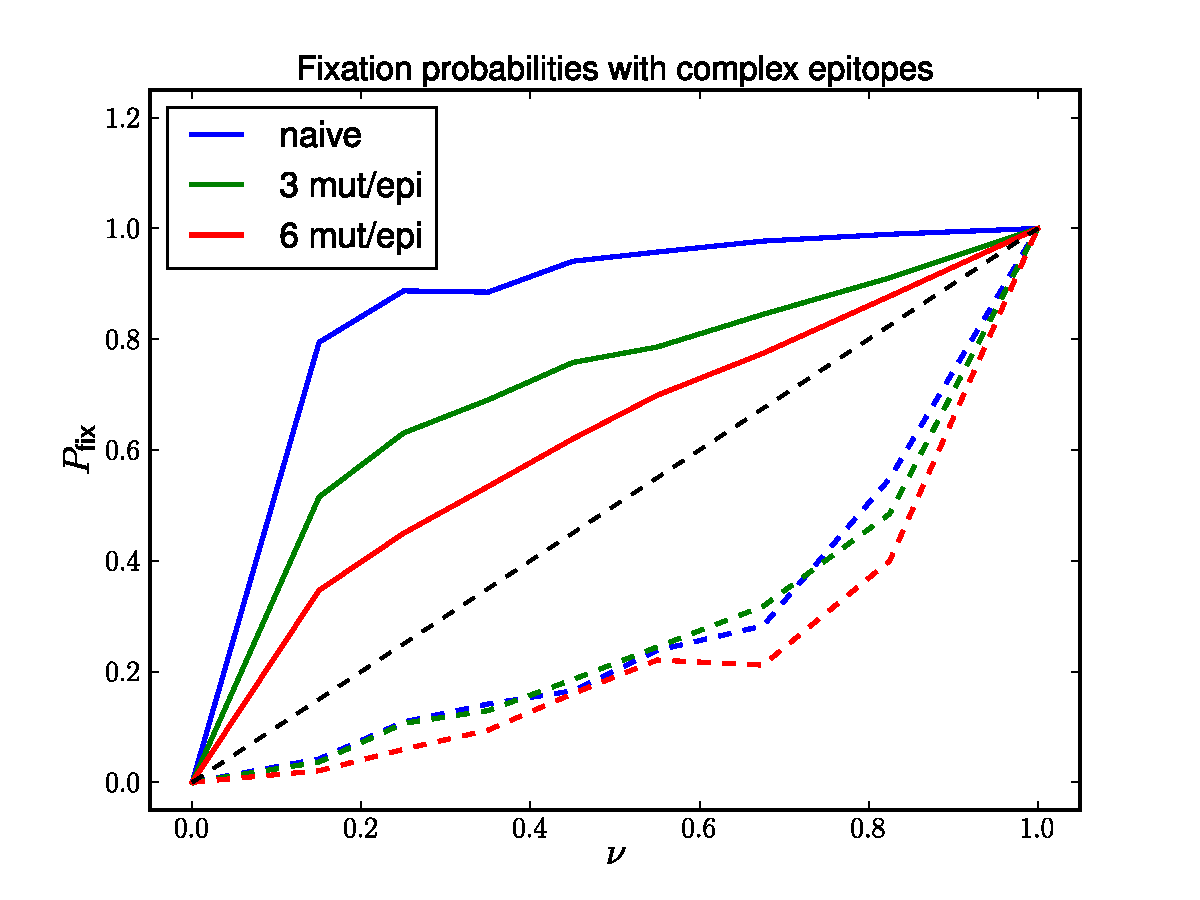
\includegraphics[width=0.6\linewidth]{simulations_gradually_epitopes}
\caption{
Competition between escape mutations in the same epitope reduces fixation of
nonsynonymous mutations. The figure compares the fixation probability of models
with one, three, or six mutually exclusive escape mutations within the
same epitope. Within epitope competition results reduced fixation
probabilities of nonsynonymous changes, whereas the synonymous changes behave 
similarly in all cases. We assume that escape can happen at $n$ sites out of 3
consecutive codons and vary $n$.
The fitness landscape of each epitope includes negative epistatic terms, so that
the joint presence of more than one escape mutation is not any more beneficial
for the virus than a single mutation. Specifically, each site has two alleles,
$\pm 1$, where $-1$ is the ancestral one and $+1$ the derived one; the fitness
coefficient of a $k$-tuple of sites within the epitope is $f_k = (-1)^{k-1}
2^{1-n}\eta_\epsilon $, where $\eta_\epsilon$ is the escape rate of the epitope
drawn from an exponential distribution with mean $\epsilon$, 
$n$ is the number of competing escapes in the epitope. 
In this evolutionary scenario, many escape mutations start to sweep on different backgrounds within the viral population, but eventually
compete and only one of them fixes. The other parameters for the shown simulations are
the following: deleterious effect $s_d = 10^{-3}$, average escape rate $\epsilon = 0.016$,
fraction of deleterious synonymous mutations $\alpha = 0.986$, rate of new epitopes
$k_A=0.0014$ per generation.
}
\label{fig:wec}
\end{center}
\end{figure}
